\chapter{Очевидности и капитальности}

По лекции от 8 сентября 2011 года.

\section{Лектор}

{\large Федор Владимирович Петров}
\par\bigskip

e-mails : \hfill fedyapetrov@gmail.com
\par\bigskip

\section{Очевидности}

\begin{Def}
	Граф - двойка $ (V , E) $, где $ V $ - конечное множество (множество вершин) и $ E \subset V^2 $ - конечное множество (множество ребер)
\end{Def}

\begin{Def}
	Граф называется неориентированным, если $ \forall (w,v \in V) \left [ (w, v) \in E \Leftrightarrow (v, w) \in E \right ] $, т. е. с каждым ребром $ (w, v) $ содержит также ребро $ (v, w) $ (таким образом направление ребра можно не учитывать). В противном случае граф называется ориентированным или орграфом.
\end{Def}

\begin{Def}
	Ребро графа вида $ (v, v) $ называется петлей.
\end{Def}

\begin{Def}
	Граф с кратными ребрами - двойка $ ( V, f ) $, где $ V $ - множество вершин, а $ f: V^2 \rightarrow \mathbb{Z _+} $ - функция кратности ребра
\end{Def}

\paragraph{Примечание}

Большую часть курса будут рассматриваться неориентированные графы без петель.

\begin{Def}
	Степенью вершины $deg (v \in V)$ неориентированного графа $ G = (V,E) $ называется число инцедентных ей ребер, т. е. \[ deg (v \in V) = \left| \{ w \in V : (w, v) \in E \lor (v, w) \in E \} \right| \]
\end{Def}

\begin{Def}
	Входной степенью вершины $ deg _{IN} (v \in V)$ ориентированного графа $ G = (V,E) $ называется число ребер заканчивающихся в этой вершине, т. е. \[ deg _{IN} (v \in V) = \left| \{ w \in V : (w, v) \in E \} \right| \]
\end{Def}

\begin{Def}
	Выходной степенью вершины $ deg _{OUT} (v \in V)$ ориентированного графа $ G = (V,E) $ называется число ребер начинающихся в этой вершине, т. е. \[ deg _{OUT} (v \in V) = \left| \{ w \in V : (v, w) \in E \} \right| \]
\end{Def}

\paragraph{Примечание}

Степень вершины может быть нулевой.

\begin{Def}
	Множество пар $ \{ (v_1, v_2), (v_2, v_3), ... , (v_{k-1}, v_{k}) $ - образуют путь, $ v_1 $ - начало пути, а $ v_k $ - конец пути
\end{Def}

\begin{Def}
	Путь, в котором начальная и конечная вершина совпадают, называется циклом
\end{Def}

\begin{Def}
	В неориентированной графе вершины $ v_i, v_j \in V $ называются связыми, если их связывает путь.
	В орграфе вершины $ v_i, v_j \in V $ называются связыми, если существуют одновременно путь из $ v_i $ в $ v_j $ и путь из $ v_j $ в $ v_i $
\end{Def}

\begin{Def}
	Если все ершины пути, кроме, быть может, первой и последней, различны, то путь (цикл) называется простым
\end{Def}

\begin{Def}
	Отношением эквивалентности на множестве называется любое отношение удовлетворяющее условиям:

\begin{itemize}
\item Рефлексивности

\item Транзитивности

\item Симметричности
\end{itemize}
\end{Def}

\section{Капитальности}

\begin{Th}
	Пусть $ G $ - граф, тогда для него выполняется соотношение \[ \sum_{v \in V} deg (v) = 2 \left| E \right| \]
\end{Th}

\begin{Proof}
	\[
		\mathfrak{1}_x =
		\begin{cases}
			1, & \text{если $x$ истинно;} \\
			0, & \text{иначе.}
		\end{cases}
	\]

	Тогда сумма степеней вершин выражается как

	\[
		\sum_{v \in V} \sum_{e \in E} \mathfrak{1}_{v \in e} = \sum_{e \in E} \sum_{v \in V} \mathfrak{1}_{v \in e} = \sum_{e \in E} 2 = 2 \left| E \right|
	\]
\end{Proof}

\paragraph{Примечание}

Для орграфа \[ \sum_{v \in V} deg_{IN} (v) = \sum_{v \in V} deg_{OUT} (v) = \left| E \right| \]

\begin{Th}
	Пусть $ X $ - множество, а $ R $ - отношение эквивалентности на элементах $ X $. $ C_x = \{ k \in X : x R k \} $ - класс эквивалентности. Тогда справедливо утверждение \[ \left( \forall x,y \in X \right) \left[ \left( C_x = C_y \right) \lor \left( C_x \cap C_y = \emptyset \right) \right] \]
\end{Th}

\begin{Proof}
	Предположим противное, что $ C_x $ и $ С_y $ - различные классы эквивалентности, которые имеют общий элемент $ z $. Тогда пользуясь свойствами отношения экивалентности:
\[
	\left( x R z \right) \land \left( y R z \right) \Leftrightarrow \left( x R z\right) \land \left( z R y \right) \Rightarrow \left( x R y \right)
\]
	Теперь возьмем произольный элемент $ w \in C_x $, получается
\[
	\left( w R x \right) \land \left( x R y \right) \Rightarrow \left( w R y \right)
\]
	Т. е. любой элемент $ w \in C_x $ одновременно содержится в $ C_y $, а так как мы не делали никаких предположений относительно классов эквивалентности, то аналогичное доказательство будет справедливо и в обратную сторону
\end{Proof}

\begin{Def}
	Множество классов эквивалентности множества $X$ по отношению $R$ - фактормножество $X/R$
\end{Def}

\begin{Def}
	Неориентированный граф $G$ - связный граф, если любая пара его вершин связана путем.
	Про орграф в этом случае, обычно, говорят, что он сильно связный.
\end{Def}

\begin{Th}
	Отношение связности двух вершин графа (орграфа) задает отношение эквивалентности. А класс эквивалентности по этому отношению называется компонентой связности (сильной связности) графа.
\end{Th}

\begin{Def}
Три определения дерева:

\begin{enumerate}
\item Граф, между любыми двумя вершинами которого сущесвует, причем единственный, простой путь.

\item Связный граф без простых циклов (на самом деле без любых).

\item Связный граф, для которого выполняется соотношение $\left| E \right| = \left| V \right| - 1$
\end{enumerate}
\end{Def}

\begin{Th}
	Определения 1 и 2 равносильны.
\end{Th}

\begin{Proof}
	Докажем, что $ 1 \Rightarrow 2 $. Очевидно, что для 2 вершин входящих в один цикл существует как минимум 2 пути из одной в другую, получается, что дерево по определению 1 не может содержать циклов.

\begin{figure}[h]
	\noindent\center{
		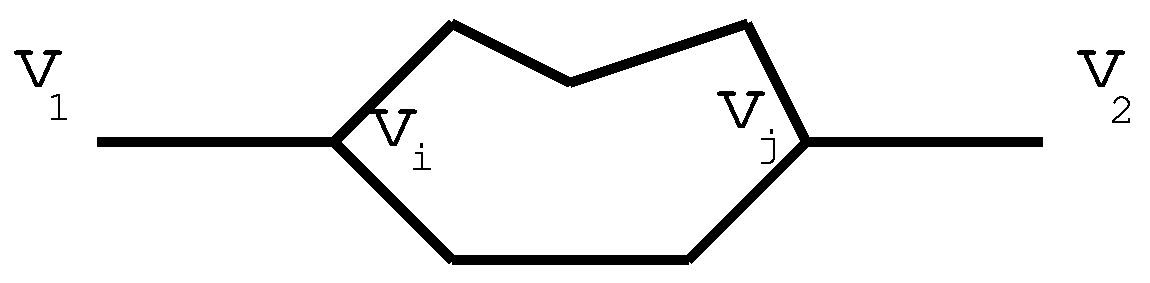
\includegraphics[width=0.5\linewidth]{simp_circle}
	}
	\caption{Выделение простого цикла}
	\label{pic::simp_circle}
\end{figure}

	Докажем, что $ 2 \Rightarrow 1 $. Пусть из вершины $ v_1 $ существует более одного пути в вершину $ v_2 $, идем по этим путям из ввершины $ v_1 $ в точку $ v_i $ (см. рис. \ref{pic::simp_circle}), в которой они расходятся (в крайнем случае $ v_1 = v_i $), далее идем уже по каждому пути до первой точки $ v_j $, в которой они сходятся (в крайнем случае $ v_j = v_2 $), образуем простой цикл, следовательно, если имеется больше одного пути между парой вершин, то в графе содержится простой цикл. 
\end{Proof}

\begin{Lem}
	В дереве, всмысле определений 1 и 2, существует как минимум 2 исящие вершины.
\end{Lem}

\begin{Proof}
	Выберем самый длинный путь в графе. Рассмотрим концы этого пути, из них не может вести ребро в точку не входящую в путь, т. к. тогда включив его в путь, мы бы получили путь длиннее самого длинного, кроме того, из них не может вести ребро в точку входящую в путь, т. к. в этом случае получится цикл, что противоречит определению 2, следовательно концы этого пути - висящие вершины графа.
\end{Proof}

\begin{Th}
	Из связного графа $G$ с циклами, удалением ребер можно получить дерево (остовное дерево).
\end{Th}

\begin{Proof}
	Фиксируем вершину графа, присваиваем ей вес 0. Далее перебираем все соседние вершины графа присваивая каждой из них вес 1. Теперь для каждой полученной вершины просматриваем непосещенных соседей, и присваиваем им вес на единицу больший, чем вес вершины (отмечаем вершину и ведущее в нее ребро). Т. к. число вершин графа конечно, то таким образом мы переберем и отметим все вершины, т. к. каждая вершина посещяется (и взвешивается) только один раз, то в полученном подграфе нет циклов. (Метод называется ранжированием, смотрите алгоритмы посика остовных деревьев)
\end{Proof}

\begin{Th}
	Определения 1 и 2 равносильны определению 3.
\end{Th}

\begin{Proof}
	Докажем, что из определений 1 и 2 следует 3. База индукции - граф из одной вершины, для которого соотношение очевидно выполняется ( $ \left| V \right| = 1 $ и $ \left| E \right| = 0 $ ).

	Пусть $ G $ - дерево, у которого $ \left| V \right| = n $, тогда  нем должно быть как минимум де висяцие вершины, удалим одну из них (и инцедентное ей ребро), получаем граф $ \tilde G $, в который по индукционному переходу удолетворяет определению 3, а значит для $ G $ оно также справедливо, т. к. они отличаются й ребром и одной вершиной.

	Докажем, что из определения 3 следуют определения 2 и 1. Пусть $ G $ - граф с циклами, удаляем последовательно ребра входящие в какой-либо цикл, при таком удалении количество вершин сохраняется. В конечном итоге мы разомкнем все циклы и получим дерево, а для дерева справедливо (как мы уже доказали) $ \left| E \right| = \left| V \right| - 1 $, а следовательно для исходного графа с циклами это соотношение не выполнялось.
\end{Proof}

\paragraph{Следствие 1.} Для любого связного графа $G$ справедливо $ \left| E(G) \right| \ge \left| V(G) \right| - 1 $

\paragraph{Следствие 2.} Если $ \left| V(G) \right| \ge 2 $, тогда в графе существует как минимум 2 вершины, удаление одной из которых (и инцедентного ребра) сохраняет связность
